\providecommand{\HomA}{\mathrm{Hom}_{A}}
\providecommand{\HomB}{\mathrm{Hom}_{B}}
\providecommand{\HomC}{\mathrm{Hom}_{C}}
\providecommand{\HomD}{\mathrm{Hom}_{D}}
\providecommand{\HomE}{\mathrm{Hom}_{E}}
\providecommand{\Nearrow}{\rotatebox[origin=c]{45}{$\Rightarrow$}}

\section{逐点右\trKanExtension{}与左\trKanExtension}\label{sec:pointwise-right-and-left-kan-extensions}

在本节中，我们对\trInfinityCategory{}之间的\trFunctor{}给出逐点右%
\trKanExtension{}的四个定义，并证明它们相互等价。我们的证明揭示，右扩张的
一般的 2-范畴式概念（见\cref{def:two-categorical-extension}）就其自身而言
过于微弱。逐点左\trKanExtension{}的对偶理论已由\cref{lem:embedded-extension-lifting}预先展示（见\cref{ex:pointwise-left-extensions}）。

\begin{definition}[扩张对粘贴的稳定性]\label{def:stable-under-pasting}
2-范畴中的一个右扩张图表 $\nu\colon rk\Rightarrow f$ 称为\textbf{与方块
$\alpha$ 粘贴稳定}（stable under pasting with a square），若粘贴复合
\begin{rveq}\label{eq:pasted-composite}
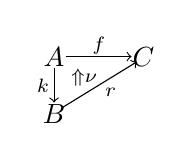
\begin{tikzpicture}[x=0.95em,y=0.95em]
  \node at (0,2.2) {$A$};
  \node at (3.4,2.2) {$C$};
  \node at (0,0) {$B$};
  \draw[->] (0.45,2.2) -- (2.95,2.2);
  \node at (1.7,2.62) {$\scriptstyle f$};
  \draw[->] (0,1.75) -- (0,0.45);
  \node at (-0.42,1.1) {$\scriptstyle k$};
  \draw[->] (0.3,0.25) -- (3.15,2.0);
  \node at (2.15,0.85) {$\scriptstyle r$};
  \node at (1.15,1.4) {$\scriptstyle\Uparrow\nu$};
\end{tikzpicture}
\qquad
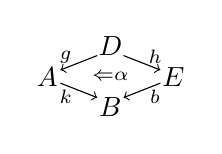
\begin{tikzpicture}[x=0.95em,y=0.95em]
  \node at (0,2.3) {$D$};
  \node at (-2.4,1.15) {$A$};
  \node at (2.4,1.15) {$E$};
  \node at (0,0) {$B$};
  \draw[->] (-0.5,1.95) -- (-1.9,1.4);
  \node at (-1.7,1.9) {$\scriptstyle g$};
  \draw[->] (0.5,1.95) -- (1.9,1.4);
  \node at (1.7,1.9) {$\scriptstyle h$};
  \draw[->] (-1.9,0.9) -- (-0.5,0.35);
  \node at (-1.7,0.4) {$\scriptstyle k$};
  \draw[->] (1.9,0.9) -- (0.5,0.35);
  \node at (1.7,0.4) {$\scriptstyle b$};
  \node at (0,1.15) {$\scriptstyle\Leftarrow\alpha$};
\end{tikzpicture}
\qquad
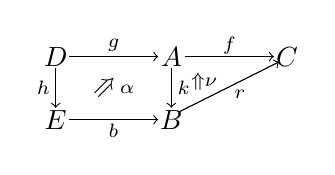
\begin{tikzpicture}[x=0.95em,y=0.95em]
  \node at (0,2.4) {$D$};
  \node at (4.4,2.4) {$A$};
  \node at (8.8,2.4) {$C$};
  \node at (0,0) {$E$};
  \node at (4.4,0) {$B$};
  \draw[->] (0.5,2.4) -- (3.9,2.4);
  \node at (2.2,2.82) {$\scriptstyle g$};
  \draw[->] (4.9,2.4) -- (8.3,2.4);
  \node at (6.6,2.82) {$\scriptstyle f$};
  \draw[->] (0,1.95) -- (0,0.45);
  \node at (-0.47,1.2) {$\scriptstyle h$};
  \draw[->] (4.4,1.95) -- (4.4,0.45);
  \node at (4.87,1.2) {$\scriptstyle k$};
  \draw[->] (0.5,0) -- (3.9,0);
  \node at (2.2,-0.42) {$\scriptstyle b$};
  \draw[->] (4.7,0.3) -- (8.5,2.2);
  \node at (7.0,0.95) {$\scriptstyle r$};
  \node at (2.2,1.2) {$\scriptstyle\Nearrow\alpha$};
  \node at (5.65,1.45) {$\scriptstyle\Uparrow\nu$};
\end{tikzpicture}
\end{rveq}
定义 $fg\colon D\to C$ 沿 $h\colon D\to E$ 的右扩张 $rb\colon E\to C$。
\end{definition}

\begin{theorem}[逐点右扩张]\label{thm:pointwise-right-extensions}
对\trInfinityCosmos{} $\mathcal{K}$ 的\trHomotopyTwoCategory{}中如下图所示的
图表，下列诸条等价：
\begin{center}
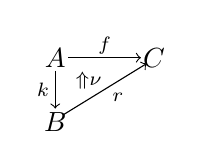
\begin{tikzpicture}[x=1.05em,y=1.05em]
  \node at (0,2.2) {$A$};
  \node at (3.4,2.2) {$C$};
  \node at (0,0) {$B$};
  \draw[->] (0.45,2.2) -- (2.95,2.2);
  \node at (1.7,2.62) {$\scriptstyle f$};
  \draw[->] (0,1.75) -- (0,0.45);
  \node at (-0.42,1.1) {$\scriptstyle k$};
  \draw[->] (0.3,0.25) -- (3.15,2.0);
  \node at (2.15,0.85) {$\scriptstyle r$};
  \node at (1.15,1.4) {$\scriptstyle\Uparrow\nu$};
\end{tikzpicture}
\end{center}
\begin{enumerate}[label=(\roman*)]
\item $\nu\colon rk\Rightarrow f$ 在 $\mathfrak{h}\mathcal{K}$ 中定义一个与%
\trExactSquare{}粘贴稳定的右扩张。
\item $\nu\colon rk\Rightarrow f$ 在 $\mathfrak{h}\mathcal{K}$ 中定义一个与%
\trCommaSquare{}粘贴稳定的右扩张。
\item $\nu_{*}\colon \HomB(B,k)\divideontimes\HomC(C,r)\Rightarrow\HomC(C,f)$
在 $\mathbb{M}od(\mathcal{K})$ 中定义一个右扩张。
\item 对任何\trExactSquare
\begin{center}
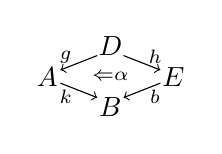
\begin{tikzpicture}[x=0.95em,y=0.95em]
  \node at (0,2.3) {$D$};
  \node at (-2.4,1.15) {$A$};
  \node at (2.4,1.15) {$E$};
  \node at (0,0) {$B$};
  \draw[->] (-0.5,1.95) -- (-1.9,1.4);
  \node at (-1.7,1.9) {$\scriptstyle g$};
  \draw[->] (0.5,1.95) -- (1.9,1.4);
  \node at (1.7,1.9) {$\scriptstyle h$};
  \draw[->] (-1.9,0.9) -- (-0.5,0.35);
  \node at (-1.7,0.4) {$\scriptstyle k$};
  \draw[->] (1.9,0.9) -- (0.5,0.35);
  \node at (1.7,0.4) {$\scriptstyle b$};
  \node at (0,1.15) {$\scriptstyle\Leftarrow\alpha$};
\end{tikzpicture}
\end{center}
$(\nu g\cdot r\alpha)_{*}\colon \HomE(E,h)\divideontimes\HomC(C,rb)\Rightarrow\HomC(C,fg)$
在 $\mathbb{M}od(\mathcal{K})$ 中定义一个右扩张。
\end{enumerate}
当这些条件成立时，我们称 $r\colon B\to C$ 定义了 $f\colon A\to C$ 沿
$k\colon A\to B$ 的一个\textbf{逐点右扩张}（pointwise right extension）。
\end{theorem}

\begin{proof}
\cref{lem:comma-squares-exact}证明了 (i)$\Rightarrow$(ii)。

为证 (ii)$\Rightarrow$(iii)，设 $\nu\colon rk\Rightarrow f$ 在
$\mathfrak{h}\mathcal{K}$ 中定义一个与\trCommaSquare{}粘贴稳定的右扩张，并考虑
$\mathbb{M}od(\mathcal{K})$ 中的一个\trCell
\begin{center}
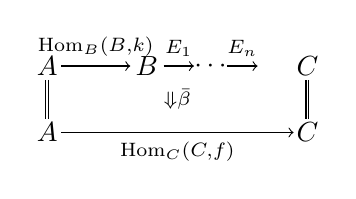
\begin{tikzpicture}[x=1.0em,y=1.0em]
  \node at (0,1.2) {$A$};
  \node at (3.6,1.2) {$B$};
  \node at (5.9,1.2) {$\cdots$};
  \node at (9.4,1.2) {$C$};
  \draw[->] (0.5,1.2) -- node[above]{$\scriptstyle\HomB(B,k)$} (3.0,1.2);
  \draw[->] (4.2,1.2) -- node[above]{$\scriptstyle E_{1}$} (5.3,1.2);
  \draw[->] (6.5,1.2) -- node[above]{$\scriptstyle E_{n}$} (7.6,1.2);
  \node at (0,-1.2) {$A$};
  \node at (9.4,-1.2) {$C$};
  \draw[->] (0.5,-1.2) -- node[below]{$\scriptstyle\HomC(C,f)$} (8.9,-1.2);
  \draw[double,double distance=0.6pt] (0,0.7) -- (0,-0.7);
  \draw[double,double distance=0.6pt] (9.4,0.7) -- (9.4,-0.7);
  \node at (4.7,0) {$\scriptstyle\Downarrow\bar{\beta}$};
\end{tikzpicture}
\end{center}
令 $B\overset{q}{\twoheadleftarrow}\vec{E}\overset{p}{\twoheadrightarrow}C$
表示复合双侧纤维化 $E_{1}\divideontimes\cdots\divideontimes E_{n}$。
由注 8.3.12，模映射
\begin{equation*}
\bar{\beta}\colon \HomB(B,k)\divideontimes E_{1}\divideontimes\cdots\divideontimes E_{n}\Rightarrow\HomC(C,f)
\end{equation*}
对应于模映射
\begin{equation*}
\hat{\beta}\colon \HomB(B,k)\divideontimes\HomB(q,B)\divideontimes\HomC(C,p)\Rightarrow\HomC(C,f).
\end{equation*}
由推论 8.4.6 与命题 8.4.7，这类模映射与模映射
\begin{equation*}
\check{\beta}\colon \HomB(q,k)\Rightarrow\HomC(p,f)
\end{equation*}
处于双射之中。由引理 8.1.16，这些模映射与\trHomotopyTwoCategory{}中的如下
2-\trCell{}一一对应
\begin{center}
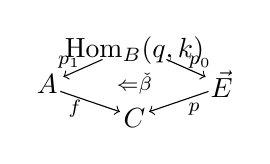
\begin{tikzpicture}[x=1.05em,y=1.05em]
  \node at (0,2.3) {$\HomB(q,k)$};
  \node at (-3.0,1.15) {$A$};
  \node at (3.0,1.15) {$\vec{E}$};
  \node at (0,0) {$C$};
  \draw[->] (-1.1,2.0) -- (-2.45,1.4);
  \node at (-2.25,1.9) {$\scriptstyle p_{1}$};
  \draw[->] (1.1,2.0) -- (2.45,1.4);
  \node at (2.25,1.9) {$\scriptstyle p_{0}$};
  \draw[->] (-2.55,0.9) -- (-0.5,0.2);
  \node at (-2.05,0.3) {$\scriptstyle f$};
  \draw[->] (2.55,0.9) -- (0.5,0.2);
  \node at (2.05,0.3) {$\scriptstyle p$};
  \node at (0,1.15) {$\scriptstyle\Leftarrow\check{\beta}$};
\end{tikzpicture}
\end{center}

由假设 (ii)，图表
\begin{center}
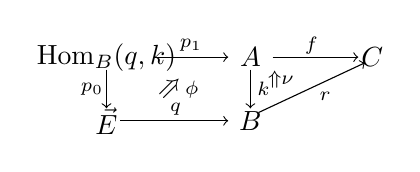
\begin{tikzpicture}[x=1.0em,y=1.0em]
  \node at (0,2.3) {$\HomB(q,k)$};
  \node at (5.2,2.3) {$A$};
  \node at (9.6,2.3) {$C$};
  \node at (0,0) {$\vec{E}$};
  \node at (5.2,0) {$B$};
  \draw[->] (1.7,2.3) -- (4.4,2.3);
  \node at (3.05,2.72) {$\scriptstyle p_{1}$};
  \draw[->] (6.0,2.3) -- (9.1,2.3);
  \node at (7.4,2.72) {$\scriptstyle f$};
  \draw[->] (0,1.85) -- (0,0.45);
  \node at (-0.52,1.15) {$\scriptstyle p_{0}$};
  \draw[->] (0.5,0) -- (4.4,0);
  \node at (2.5,0.4) {$\scriptstyle q$};
  \draw[->] (5.2,1.85) -- (5.2,0.45);
  \node at (5.67,1.15) {$\scriptstyle k$};
  \draw[->] (5.5,0.3) -- (9.35,2.1);
  \node at (7.9,0.9) {$\scriptstyle r$};
  \node at (2.6,1.15) {$\scriptstyle\Nearrow\phi$};
  \node at (6.3,1.5) {$\scriptstyle\Uparrow\nu$};
\end{tikzpicture}
\end{center}
在 $\mathfrak{h}\mathcal{K}$ 中定义一个右扩张，于是 $\beta$ 经由一个%
\trNaturalTransformation{} $\gamma\colon p\Rightarrow rq$ 唯一地分解过这一
粘贴复合。由命题 8.4.11，这就定义了一个胞腔
$\gamma_{*}\colon \HomC(C,p)\Rightarrow\HomC(C,rq)$，而由推论 8.4.6，它给出
一个\trCanonical{}胞腔
$\hat{\gamma}\colon \HomB(q,B)\divideontimes\HomC(C,p)\Rightarrow\HomC(C,r)$。
再次由注 8.3.12，这就产生了所要的那个唯一分解
\begin{center}
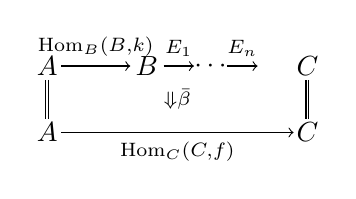
\begin{tikzpicture}[x=1.0em,y=1.0em]
  \node at (0,1.2) {$A$};
  \node at (3.6,1.2) {$B$};
  \node at (5.9,1.2) {$\cdots$};
  \node at (9.4,1.2) {$C$};
  \draw[->] (0.5,1.2) -- node[above]{$\scriptstyle\HomB(B,k)$} (3.0,1.2);
  \draw[->] (4.2,1.2) -- node[above]{$\scriptstyle E_{1}$} (5.3,1.2);
  \draw[->] (6.5,1.2) -- node[above]{$\scriptstyle E_{n}$} (7.6,1.2);
  \node at (0,-1.2) {$A$};
  \node at (9.4,-1.2) {$C$};
  \draw[->] (0.5,-1.2) -- node[below]{$\scriptstyle\HomC(C,f)$} (8.9,-1.2);
  \draw[double,double distance=0.6pt] (0,0.7) -- (0,-0.7);
  \draw[double,double distance=0.6pt] (9.4,0.7) -- (9.4,-0.7);
  \node at (4.7,0) {$\scriptstyle\Downarrow\bar{\beta}$};
\end{tikzpicture}
\quad$=$\quad
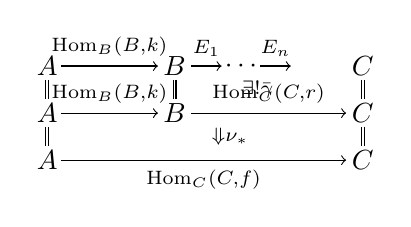
\begin{tikzpicture}[x=1.0em,y=1.0em]
  \node at (0,3.4) {$A$};
  \node at (4.6,3.4) {$B$};
  \node at (7.0,3.4) {$\cdots$};
  \node at (11.4,3.4) {$C$};
  \draw[->] (0.5,3.4) -- node[above]{$\scriptstyle\HomB(B,k)$} (4.0,3.4);
  \draw[->] (5.2,3.4) -- node[above]{$\scriptstyle E_{1}$} (6.3,3.4);
  \draw[->] (7.7,3.4) -- node[above]{$\scriptstyle E_{n}$} (8.8,3.4);
  \node at (0,1.7) {$A$};
  \node at (4.6,1.7) {$B$};
  \node at (11.4,1.7) {$C$};
  \draw[->] (0.5,1.7) -- node[above]{$\scriptstyle\HomB(B,k)$} (4.0,1.7);
  \draw[->] (5.2,1.7) -- node[above]{$\scriptstyle\HomC(C,r)$} (10.8,1.7);
  \node at (0,0) {$A$};
  \node at (11.4,0) {$C$};
  \draw[->] (0.5,0) -- node[below]{$\scriptstyle\HomC(C,f)$} (10.8,0);
  \draw[double,double distance=0.6pt] (0,2.9) -- (0,2.2);
  \draw[double,double distance=0.6pt] (0,1.2) -- (0,0.5);
  \draw[double,double distance=0.6pt] (4.6,2.9) -- (4.6,2.2);
  \draw[double,double distance=0.6pt] (11.4,2.9) -- (11.4,2.2);
  \draw[double,double distance=0.6pt] (11.4,1.2) -- (11.4,0.5);
  \node at (7.6,2.55) {$\scriptstyle\exists!\bar{\gamma}$};
  \node at (6.6,0.85) {$\scriptstyle\Downarrow\nu_{*}$};
\end{tikzpicture}
\end{center}

为证 (iii)$\Rightarrow$(iv)，考虑一个使 $\alpha\colon bh\Rightarrow kg$
为正合、且 $\nu_{*}\colon \HomB(B,k)\divideontimes\HomC(C,r)\Rightarrow\HomC(C,f)$
在 $\mathbb{M}od(\mathcal{K})$ 中定义一个右扩张图表的图表
\eqref{eq:pasted-composite}。现在由推论 8.4.6，一个胞腔
\begin{equation*}
\bar{\beta}\colon \HomE(E,h)\divideontimes E_{1}\divideontimes\cdots\divideontimes E_{n}\Rightarrow\HomC(C,fg)
\end{equation*}
对应于一个胞腔
\begin{equation*}
\hat{\beta}\colon \HomA(g,A)\divideontimes\HomE(E,h)\divideontimes E_{1}\divideontimes\cdots\divideontimes E_{n}\Rightarrow\HomC(C,f).
\end{equation*}
由 $\alpha$ 的正合性，这对应于一个胞腔
\begin{equation*}
\hat{\beta}\colon \HomB(b,k)\divideontimes E_{1}\divideontimes\cdots\divideontimes E_{n}\Rightarrow\HomC(C,f),
\end{equation*}
或者等价地，沿复合映射
$\circ\colon \HomB(B,k)\divideontimes\HomB(b,B)\Rightarrow\HomB(b,k)$ 作限制，得到
一个胞腔
\begin{equation*}
\hat{\beta}\colon \HomB(B,k)\divideontimes\HomB(b,B)\divideontimes E_{1}\divideontimes\cdots\divideontimes E_{n}\Rightarrow\HomC(C,f).
\end{equation*}
由于 $B\xrightarrow{\HomC(C,r)}C$ 是 $A\xrightarrow{\HomC(C,f)}C$ 沿
$A\xrightarrow{\HomB(B,k)}B$ 的右扩张，这对应于一个胞腔
\begin{equation*}
\hat{\gamma}\colon \HomB(b,B)\divideontimes E_{1}\divideontimes\cdots\divideontimes E_{n}\Rightarrow\HomC(C,r),
\end{equation*}

它经由推论 8.4.6 转置为一个胞腔
\begin{equation*}
\bar{\gamma}\colon E_{1}\divideontimes\cdots\divideontimes E_{n}\Rightarrow\HomC(C,rb),
\end{equation*}
这就给出了证明模块 $E\xrightarrow{\HomC(C,rb)}C$ 是
$D\xrightarrow{\HomC(C,fg)}C$ 沿 $D\xrightarrow{\HomE(E,h)}E$ 的右扩张所需的
因子分解。要看出这一双射经由与映射
$(\nu g\cdot r\alpha)_{*}\colon \HomE(E,h)\divideontimes\HomC(C,rb)\Rightarrow\HomC(C,fg)$
（即对应于粘贴复合 \eqref{eq:pasted-composite} 的那个映射）的复合来实现，
需要一个稍微精细些的论证；但为此，由\trYonedaLemma，从恒同胞腔
$\mathrm{id}_{\HomC(C,rb)}$ 出发、沿刚才描述的双射逐级向上回溯便已足够。
利用引理 8.1.16，这是直截了当的。

最后，\cref{lem:embedded-extension-lifting}与\cref{lem:trivial-exact-squares}
这一平凡例子共同证明了 (iv)$\Rightarrow$(i)。
\end{proof}

利用\cref{thm:pointwise-right-extensions}的各种刻画，我们可以建立逐点右%
扩张的一些基本稳定性性质。

\begin{corollary}\label{cor:pasting-pointwise-right-extension}
逐点右扩张与一个\trExactSquare{}的粘贴复合 \eqref{eq:pasted-composite} 仍是
一个逐点右扩张。
\end{corollary}

\begin{proof}
由\cref{lem:composites-exact-squares}，两个\trExactSquare{}的粘贴复合仍是%
\trExactSquare，故由\cref{thm:pointwise-right-extensions}(i)，逐点右扩张的
粘贴复合仍保持与正合方块粘贴稳定。
\end{proof}

\begin{corollary}\label{cor:composite-pointwise-extensions}
考虑由\trFunctor{}与\trNaturalTransformation{}构成的如下图所示的图表，其中
$(r,\nu\colon rk\Rightarrow f)$ 是 $f$ 沿 $k$ 的一个逐点右扩张。那么，
$(s,\sigma\colon sh\Rightarrow r)$ 是 $r$ 沿 $h$ 的一个逐点右扩张，当且仅当
$(s,\nu\cdot\sigma k\colon shk\Rightarrow f)$ 是 $f$ 沿 $hk$ 的一个逐点右扩张。
\begin{center}
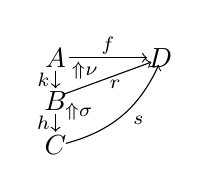
\begin{tikzpicture}[x=1.05em,y=1.05em]
  \node at (0,3.0) {$A$};
  \node at (3.6,3.0) {$D$};
  \node at (0,1.5) {$B$};
  \node at (0,0) {$C$};
  \draw[->] (0.45,3.0) -- (3.15,3.0);
  \node at (1.8,3.42) {$\scriptstyle f$};
  \draw[->] (0,2.55) -- (0,1.95);
  \node at (-0.42,2.25) {$\scriptstyle k$};
  \draw[->] (0.3,1.75) -- (3.3,2.85);
  \node at (2.05,2.1) {$\scriptstyle r$};
  \node at (1.0,2.55) {$\scriptstyle\Uparrow\nu$};
  \draw[->] (0,1.05) -- (0,0.45);
  \node at (-0.42,0.75) {$\scriptstyle h$};
  \draw[->] (0.35,0.05) to[bend right=25] (3.55,2.75);
  \node at (2.85,0.85) {$\scriptstyle s$};
  \node at (0.8,1.15) {$\scriptstyle\Uparrow\sigma$};
\end{tikzpicture}
\end{center}
\end{corollary}

\begin{proof}
由\cref{thm:pointwise-right-extensions}，\trHomotopyTwoCategory{}中的一个%
\trNaturalTransformation{}是逐点右扩张，当且仅当它到模的\trVirtualEquipment{}中的
共变嵌入是一个右扩张。
在\cref{prop:right-extension-associativity}的双射之下，二元模映射
$\sigma_{*}\colon \HomC(C,h)\divideontimes\HomD(D,s)\Rightarrow\HomD(D,r)$ 与
$(\nu\cdot\sigma k)_{*}\colon \HomC(C,hk)\divideontimes\HomD(D,s)\Rightarrow\HomD(D,f)$\footnote{原书印作
「$\HomC(hk)$」，疑脱首参，应为「$\HomC(C,hk)$」之误，此处径改。——译者注}
相互对应：
\begin{center}
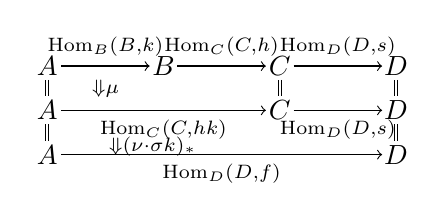
\begin{tikzpicture}[x=1.0em,y=1.0em]
  \node at (0,3.2) {$A$};
  \node at (4.2,3.2) {$B$};
  \node at (8.4,3.2) {$C$};
  \node at (12.6,3.2) {$D$};
  \draw[->] (0.5,3.2) -- node[above]{$\scriptstyle\HomB(B,k)$} (3.7,3.2);
  \draw[->] (4.7,3.2) -- node[above]{$\scriptstyle\HomC(C,h)$} (7.9,3.2);
  \draw[->] (8.9,3.2) -- node[above]{$\scriptstyle\HomD(D,s)$} (12.1,3.2);
  \node at (0,1.6) {$A$};
  \node at (8.4,1.6) {$C$};
  \node at (12.6,1.6) {$D$};
  \draw[->] (0.5,1.6) -- node[below]{$\scriptstyle\HomC(C,hk)$} (7.9,1.6);
  \draw[->] (8.9,1.6) -- node[below]{$\scriptstyle\HomD(D,s)$} (12.1,1.6);
  \node at (0,0) {$A$};
  \node at (12.6,0) {$D$};
  \draw[->] (0.5,0) -- node[below]{$\scriptstyle\HomD(D,f)$} (12.1,0);
  \draw[double,double distance=0.6pt] (0,2.7) -- (0,2.1);
  \draw[double,double distance=0.6pt] (0,1.1) -- (0,0.5);
  \draw[double,double distance=0.6pt] (8.4,2.7) -- (8.4,2.1);
  \draw[double,double distance=0.6pt] (12.6,2.7) -- (12.6,2.1);
  \draw[double,double distance=0.6pt] (12.6,1.1) -- (12.6,0.5);
  \node at (2.1,2.4) {$\scriptstyle\Downarrow\mu$};
  \node at (3.8,0.3) {$\scriptstyle\Downarrow(\nu\cdot\sigma k)_{*}$};
\end{tikzpicture}
\qquad$\mathrel{\leftrightsquigarrow}$\qquad
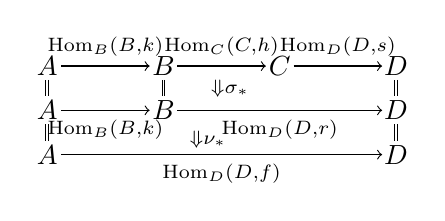
\begin{tikzpicture}[x=1.0em,y=1.0em]
  \node at (0,3.2) {$A$};
  \node at (4.2,3.2) {$B$};
  \node at (8.4,3.2) {$C$};
  \node at (12.6,3.2) {$D$};
  \draw[->] (0.5,3.2) -- node[above]{$\scriptstyle\HomB(B,k)$} (3.7,3.2);
  \draw[->] (4.7,3.2) -- node[above]{$\scriptstyle\HomC(C,h)$} (7.9,3.2);
  \draw[->] (8.9,3.2) -- node[above]{$\scriptstyle\HomD(D,s)$} (12.1,3.2);
  \node at (0,1.6) {$A$};
  \node at (4.2,1.6) {$B$};
  \node at (12.6,1.6) {$D$};
  \draw[->] (0.5,1.6) -- node[below]{$\scriptstyle\HomB(B,k)$} (3.7,1.6);
  \draw[->] (4.7,1.6) -- node[below]{$\scriptstyle\HomD(D,r)$} (12.1,1.6);
  \node at (0,0) {$A$};
  \node at (12.6,0) {$D$};
  \draw[->] (0.5,0) -- node[below]{$\scriptstyle\HomD(D,f)$} (12.1,0);
  \draw[double,double distance=0.6pt] (0,2.7) -- (0,2.1);
  \draw[double,double distance=0.6pt] (0,1.1) -- (0,0.5);
  \draw[double,double distance=0.6pt] (4.2,2.7) -- (4.2,2.1);
  \draw[double,double distance=0.6pt] (12.6,2.7) -- (12.6,2.1);
  \draw[double,double distance=0.6pt] (12.6,1.1) -- (12.6,0.5);
  \node at (6.6,2.4) {$\scriptstyle\Downarrow\sigma_{*}$};
  \node at (5.8,0.55) {$\scriptstyle\Downarrow\nu_{*}$};
\end{tikzpicture}
\end{center}
于是，由该结果\footnote{原书左图首行第二模印作「$\HomC(C,k)$」，按型算疑为
「$\HomC(C,h)$」之误，此处径改。——译者注}，$\sigma_{*}$ 是一个右扩张当且仅当
$(\nu\cdot\sigma k)_{*}$ 是一个右扩张，即如所断言。
\end{proof}

\subsection*{练习}

\begin{exercise}\label{ex:pointwise-left-extensions}
以\cref{lem:embedded-extension-lifting}为提示，陈述并证明%
\cref{thm:pointwise-right-extensions}的一个对偶版本，以定义%
\trInfinityCosmos{}的\trHomotopyTwoCategory{}中的逐点左扩张。
\end{exercise}

